% Gemini theme
% https://github.com/anishathalye/gemini

\documentclass[final]{beamer}

% ====================
% Packages
% ====================

\usepackage[T1]{fontenc}
\usepackage{lmodern}
\usepackage[size=custom,width=91.4,height=121.9,scale=1.25]{beamerposter}
\usetheme{gemini}
\usecolortheme{rpi}
\usepackage{graphicx}
\usepackage{booktabs}
\usepackage{tikz}
\usetikzlibrary{positioning,fit,calc,shapes,arrows.meta,shapes.callouts}
\usepackage{pgfkeys}
\usepackage{pgfplots}
\pgfplotsset{compat=1.14}
\usepackage{anyfontsize}

% ====================
% Lengths
% ====================

% If you have N columns, choose \sepwidth and \colwidth such that
% (N+1)*\sepwidth + N*\colwidth = \paperwidth
\newlength{\sepwidth}
\newlength{\colwidth}
\setlength{\sepwidth}{0.008\paperwidth}
\setlength{\colwidth}{0.24\paperwidth}

\newcommand{\separatorcolumn}{\begin{column}{\sepwidth}\end{column}}

% ====================
% Title
% ====================

\title{Deciphering Crypto Twitter}

\author{Inwon Kang \inst{1} \and Maruf Ahmed Mridul \inst{1} \and Abraham Sanders \inst{1} \and \\ Yao Ma \inst{1} \and Thilanka Munasinghe \inst{1} \and Aparna Gupta \inst{1} \and Oshani Seneviratne \inst{1}}

\institute[shortinst]{\inst{1} Rensselaer Polytechnic Institute}

% ====================
% Footer (optional)
% ====================

\footercontent{
	% \href{https://www.example.com}{https://www.example.com} \hfill
	WebSci-24, Stuttgart, Germany\hfill
	\href{mailto:inwon.kang04@gmail.com}{inwon.kang04@gmail.com}}
% (can be left out to remove footer)

% ====================
% Logo (optional)
% ====================

% use this to include logos on the left and/or right side of the header:
% \logoright{\includegraphics[height=7cm]{logo1.pdf}}
% \logoleft{\includegraphics[height=7cm]{logo2.pdf}}

% ====================
% CUstom Macros
% ====================

\newlength{\gap}
\newlength{\titleheight}
\newlength{\contentheight}
\newlength{\clustergap}
\newlength{\clusterwidth}

\definecolor{cluster1}{HTML}{5F67EF}
\definecolor{cluster2}{HTML}{E14630}
\definecolor{cluster3}{HTML}{52CF94}
\definecolor{cluster4}{HTML}{995FFE}
\definecolor{cluster5}{HTML}{F59A4F}
\definecolor{cluster6}{HTML}{58D6F6}
\definecolor{posblue}{HTML}{1637de}
\definecolor{bordergray}{HTML}{5c5c5c}
\definecolor{overallgray}{HTML}{adadad}
\definecolor{maintextbackground}{HTML}{C2571A}
\definecolor{maintextforeground}{HTML}{FFFFFF}
\definecolor{customorange}{HTML}{DA621E}
% \definecolor{customorange}{HTML}{DA621E}

% Define the key-value interface
\pgfkeys{
  /clusterInfo/.is family, /clusterInfo,
  default/.style = {
    key = {},
    fill = {blue},
    placement = {(0,0)},
    width = {\textwidth},
    height = {4.0em},
    gap = {0.3em},
    titleheight = {1.4em},
  },
  key/.store in = \clusterInfoKey,
  fill/.store in = \clusterInfoColor,
  placement/.store in = \clusterInfoPlacement,
  width/.store in = \clusterInfoWidth,
  height/.store in = \clusterInfoHeight,
  gap/.store in = \clusterInfoGapWidth,
  titleheight/.store in = \clusterInfoTitleHeight,
}

\newcommand{\clusterInfo}[3][]{%
  \pgfkeys{/clusterInfo, default, #1}%

  % \newlength{\cotentwidth}
  \setlength{\gap}{\clusterInfoGapWidth}
  \pgfmathsetlength{\titleheight}{\clusterInfoTitleHeight}
  \pgfmathsetlength{\contentheight}{\clusterInfoHeight-\clusterInfoTitleHeight-3\gap}

  \node[
    container,
    inner sep=0pt,
    fill=\clusterInfoColor!20,
    minimum width=\clusterInfoWidth,
    minimum height=\clusterInfoHeight
  ] (\clusterInfoKey_Box) 
  at \clusterInfoPlacement {};

  \node[
    title,
    minimum width=\clusterInfoWidth-2\gap,
    minimum height=\titleheight
  ] (\clusterInfoKey_Title)
  at ($(\clusterInfoKey_Box.north) + (0,-0.5\titleheight-\gap)$) {
    #2
  };

  \node[
    content,
    minimum width=\clusterInfoWidth-2\gap,
    minimum height=\clusterInfoHeight-\titleheight-3\gap
  ] (\clusterInfoKey_Content) 
  at ($(\clusterInfoKey_Box.north) + (0,-\titleheight-2\gap-0.5\contentheight)$) {
    \begin{minipage}{\clusterInfoWidth-4\gap}
      \vspace{0em}
      \centering
      #3
    \end{minipage}
  };
}

% ====================
% Body
% ====================

\begin{document}

% Refer to https://github.com/k4rtik/uchicago-poster
% logo: https://www.cam.ac.uk/brand-resources/about-the-logo/logo-downloads
\addtobeamertemplate{headline}{}
{
	\begin{tikzpicture}[remember picture,overlay]
		\node [anchor=north west, inner sep=0] (rpilogo)
    at ($(current page.north west) + (4em,-1.8em)$)
		{
\includegraphics[height=9em]{logo/RPI-Logo-TwoColor.png}};
		\node [anchor=north east, inner sep=0] (craftlogo)
    at ($(current page.north east) + (-4em,-1.8em)$)
		{
\includegraphics[height=9em]{logo/CRAFT_LOGO.png}};
	\end{tikzpicture}
}

\begin{frame}[t]

	\newlength{\maintextwidth}
	\newlength{\maintextheight}
	\setlength{\maintextwidth}{0.85\paperwidth}
	\setlength{\maintextheight}{10em}

	\vspace{-1em}
	\begin{tikzpicture}[%
			container/.style={
					rectangle,
					draw=bordergray,
					fill=rpi_red!80,
					rounded corners,
					inner sep=0pt,
					inner ysep=0pt,
					minimum width=\maintextwidth,
					minimum height=\maintextheight
				},
			content/.style={
					inner sep=0pt,
					inner ysep=0pt
				},
		]

		\node[rectangle,minimum width=\textwidth] (dummy)
		at (0,0) {};
		\node[container] (maintextbackground)
		at ($(dummy.north)+(0,-0.5\maintextheight-1em)$) {};

		\node[
			content,
			minimum width=\maintextwidth,
		] (maintextcontent)
		at ($(maintextbackground.north) + (0,-0.5\maintextheight)$) {
			\begin{minipage}[t]{\maintextwidth-2em}
				\vspace{0em}
				\centering
				{
					\color{maintextforeground}
					\textbf{\huge
						The rise in popularity of cryptocurrencies has led to an emergence of a new form of social media, known as \textit{Crypto Twitter}.\\
						What can this data tell us about the cryptocurrency ecosystem?
					}
				}
			\end{minipage}
		};

	\end{tikzpicture}

	\vspace{-1em}
	\begin{columns}[t]
		\begin{column}{0.01\paperwidth}\end{column}
		\begin{column}{0.73\paperwidth}
			\begin{block}{Data Collection \& Processing}
				\newlength{\gapx}
				\newlength{\gapy}
				\newlength{\boxwidth}
				\newlength{\boxheight}

				\setlength{\gapx}{1.6em}
				\setlength{\gapy}{1.2em}
				\setlength{\boxwidth}{0.2\textwidth-0.8\gapx}
				\setlength{\boxheight}{6em}

				\vspace{-3.7em}
				\begin{tikzpicture}[%
						container/.style={
								rectangle,
								draw=bordergray,
								rounded corners,
								inner sep=0pt,
								inner ysep=0pt,
								minimum width=\boxwidth,
								minimum height=\boxheight
							},
						title/.style={
							},
						content/.style={
								fill=white,
								rectangle,
								rounded corners,
								inner sep=0pt,
								inner ysep=0pt
							},
					]

					% \node[rectangle,fill=blue,minimum width=\textwidth] (dummy) at (0,0) {};
					\clusterInfo[%
						key={Collection},
						% placement={(dummy.north west)},
						placement={(0,0)},
						width={\boxwidth},
						height={\boxheight},
						titleheight={0.8em},
						fill={customorange},
					]{
						\textbf{Data Collection}
					}{
						% 
						% \hspace{1em}
						% 
					}

					\node[] (twitterlogo)
					at ($(Collection_Content.north west)+(2.2em,-2.2em)$)
					{
\includegraphics[width=3.2em]{./figures/x-logo.png}};
					\node[] (elasticsearch)
					at ($(Collection_Content.south east)+(-2.2em,2.2em)$)
					{
\includegraphics[width=3.6em]{./figures/elasticsearch.png}};

					\clusterInfo[%
						key={Processing},
						placement={(\gapx+\boxwidth,0)},
						width={\boxwidth},
						height={\boxheight},
						titleheight={0.8em},
						fill={customorange},
					]{
						\textbf{Data Processing}
					}{
						Filtering, Tokenization, Embedding
					}

					\clusterInfo[%
						key={Clustering},
						placement={(3\gapx+3\boxwidth,0)},
						width={\boxwidth},
						height={\boxheight},
						titleheight={0.8em},
						fill={customorange},
					]{
						\textbf{Tweet Clustering}
					}{
						Autoencoder, K-Search, K-Means
					}

					\draw [-Triangle, line width=0.1em]
					($(Collection_Box.east)+(0.2\gapx,0)$)
					-- ($(Processing_Box.west)+(-0.2\gapx,0)$);

					\draw[-Triangle, line width=0.1em]
					($(Processing_Box.south)+(0,-0.2\gapy)$)
					[out=-40, in=150] to
					($(Clustering_Box.north)+(0,0.2\gapy)$)
					;

					\clusterInfo[%
						key={Network},
						placement={(2\gapx+2\boxwidth,0)},
						width={\boxwidth},
						height={\boxheight},
						titleheight={0.8em},
						fill={customorange},
					]{
						\textbf{Network Analysis}
					}{
						User Graph, Reply Graph
					}

					\draw [-Triangle, line width=0.1em]
					($(Processing_Box.east)+(0.2\gapx,0)$)
					-- ($(Network_Box.west)+(-0.2\gapx,0)$);

					\clusterInfo[%
						key={Sentiment},
						placement={(4\gapx+4\boxwidth,0)},
						width={\boxwidth},
						height={\boxheight},
						titleheight={0.8em},
						fill={customorange},
					]{
						\textbf{Sentiment Analysis}
					}{
						RoBERTa, Vader, Dashboard
					}

					\draw [-Triangle, line width=0.1em]
					($(Clustering_Box.east)+(0.2\gapx,0)$)
					-- ($(Sentiment_Box.west)+(-0.2\gapx,0)$);

				\end{tikzpicture}
				\vspace{-6.2em}

				\begin{minipage}{0.44\textwidth}
					\begin{figure}
						\centering
						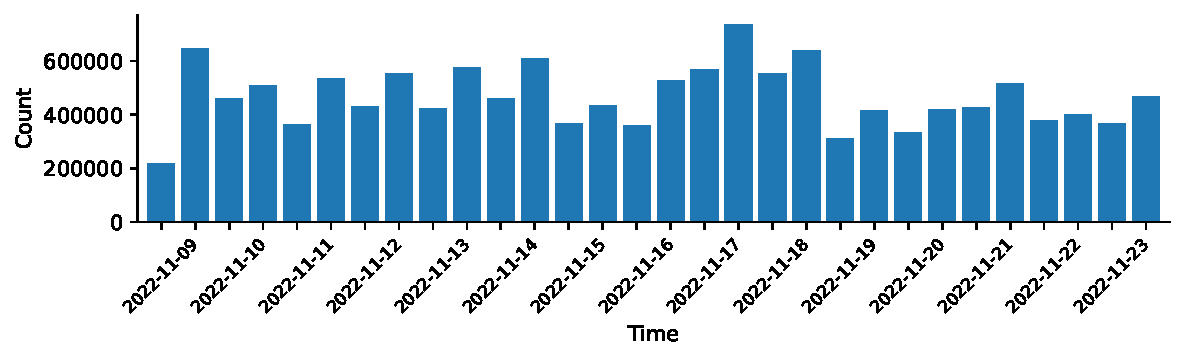
\includegraphics[width=\textwidth]{./figures/Data_Collection/tweet_volumes.pdf}
						{\color{rpi_darkgray} \small Tweet volumes over collection period. (39,828,572 total)}
					\end{figure}
				\end{minipage}
				\begin{minipage}{0.55\textwidth}
					\centering
					\begin{itemize}
						\large
						\item Tweets are collected by searching against a list of 100 hand-curated keywords about cryptocurrencies or security.
						\item Autoencoder is used to reduce the dimensionality of the BERT embeddings for clustering.
					\end{itemize}
				\end{minipage}

			\end{block}

			\vspace{-1em}
			\begin{block}{Cluster Analysis}
				\vspace{-6em}
				\begin{minipage}[t]{0.23\textwidth}
					\centering
					\vspace{0pt}
					\begin{figure}
						\centering
						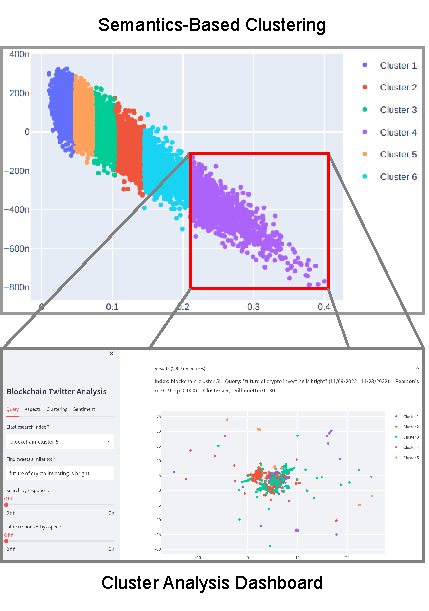
\includegraphics[width=0.95\textwidth]{./figures/Methodology//blockchain-twitter-analysis-workflow.pdf}
					\end{figure}
					\vspace{-1em}
					{\color{rpi_darkgray} \small K-Means Clustering of Tweets.}
				\end{minipage}%
				\begin{minipage}[t]{0.76\textwidth}
					\vspace{0pt}
					\centering
					{
						\large
						\begin{itemize}
							\item The tweet clusters can be characterized into on-topic, conspiracy theorists, meta discussions.
							\item Sentiment change across clusters over time show correlation to real-life events such as giveaways (airdrops) or scams.
						\end{itemize}
					}
          \vspace{1.4em}
					\begin{table}
						\centering
						{\small
							\begin{tabular}[c]{lll}
								\toprule
								\textbf{ID} & \textbf{Characterization} & \textbf{Top 10 Keywords}                                                               \\ \midrule
								            & \emph{Overall}            & \texttt{user, http, pump, just, signal, happen, crypto, wallstreetbets, event, kucoin} \\
								1           & Crypto Conspirators       & \texttt{user, pump, http, signal, just, event, happen, wallstreetbets, kucoin, big}    \\
								2           & Meta Crypto Twitter       & \texttt{user, crypto, http, promote, roll, token, price, 000, binance, security}       \\
								3           & Crypto Observers          & \texttt{user, http, crypto, v2, rollup, address, tokens, claiming, compatible, evm}    \\
								4           & Crypto Commenters         & \texttt{roll, crypto, sushi, user, project, security, good, try, http, bridge}         \\
								5           & Crypto Doubters           & \texttt{user, http, pump, crypto, just, signal, kucoin, happen, event, wallstreetbets} \\
								6           & Interested Investors      & \texttt{promote, user, crypto, price, roll, http, btc, binance, eth, bitcoin}          \\
								\bottomrule
							\end{tabular}
						}
					\end{table}
					\vspace{1.07em}
					{\color{rpi_darkgray} \small Top 10 most frequent terms of each cluster.}
				\end{minipage}%
			\end{block}
		\end{column}
		\begin{column}{0.01\paperwidth}\end{column}
		\begin{column}{0.24\paperwidth}
			\centering
			\begin{figure}
				\centering
				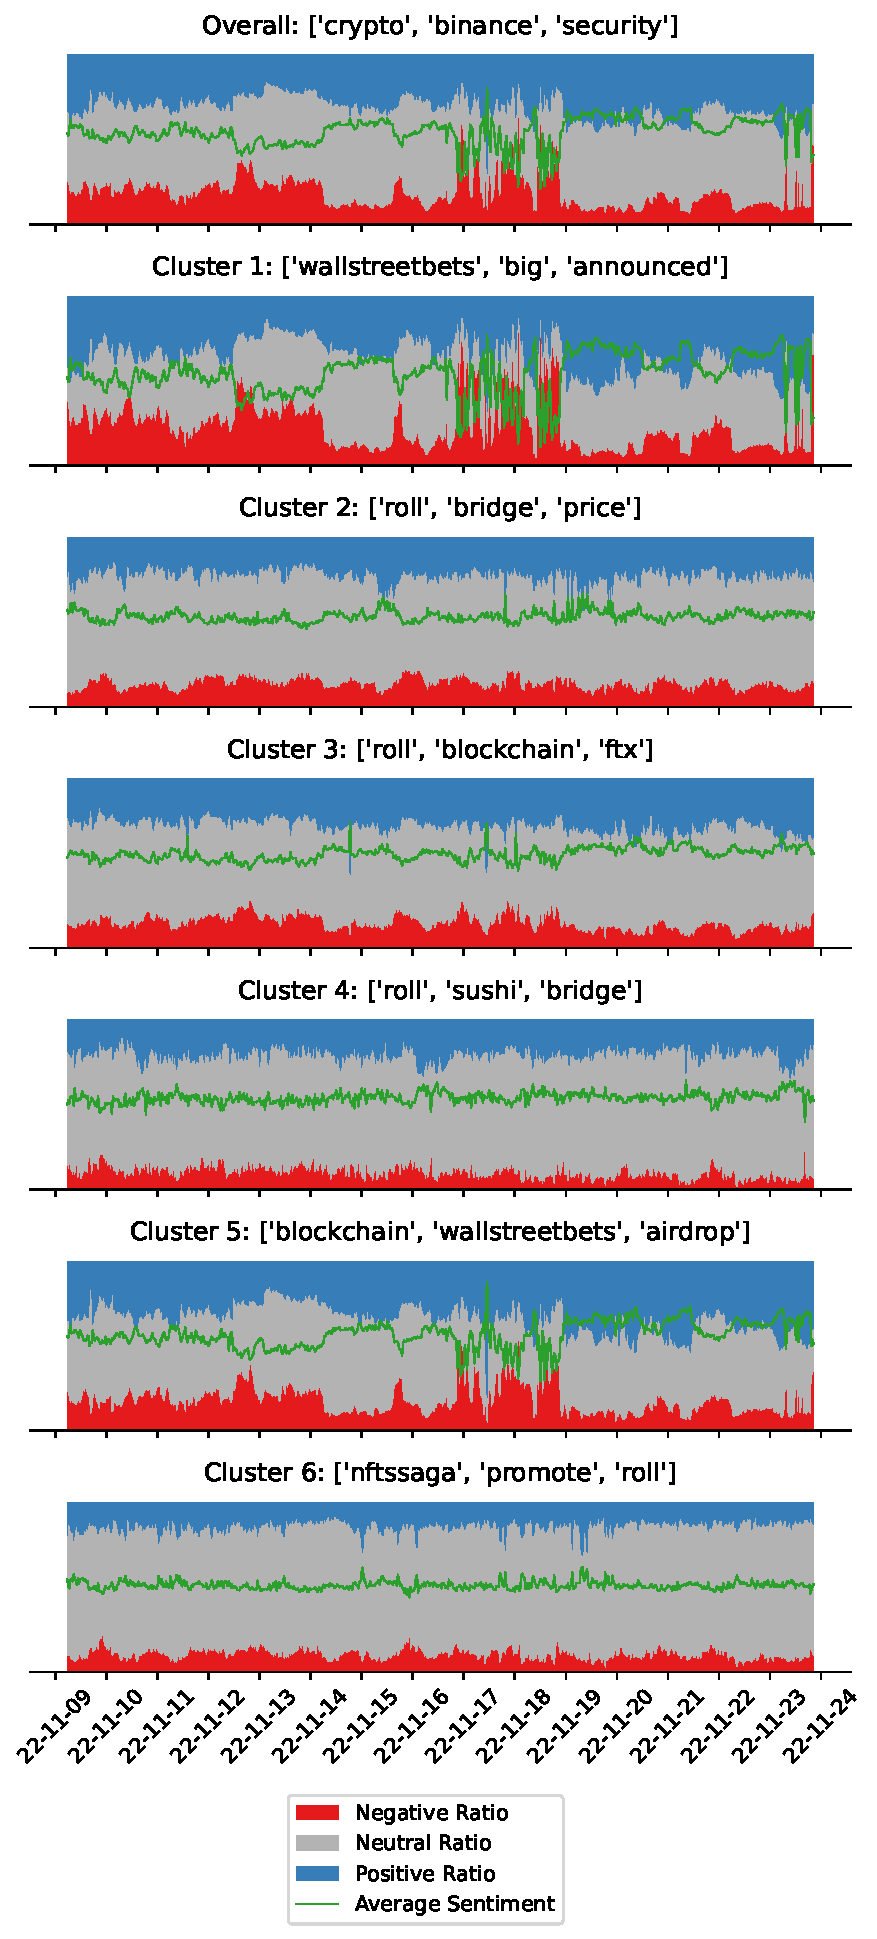
\includegraphics[width=\textwidth]{./figures/Results/sentiment/change_over_time.pdf}
			\end{figure}
			\vspace{-0.6em}
			{\color{rpi_darkgray} \small Sentiment Change Over Time.}
		\end{column}
		\begin{column}{0.01\paperwidth}\end{column}
	\end{columns}

	\vspace{-1.0em}
	\begin{columns}[t]
		\begin{column}{0.01\paperwidth}\end{column}
		\begin{column}{0.98\paperwidth}
			\begin{block}{Network Analysis}
				\vspace{-2em}
				\begin{minipage}[t]{.50\textwidth}
					\vspace{0em}
					\begin{tikzpicture}[%
							canvas/.style={
									rounded corners,
									inner sep=0pt,
									inner ysep=0pt,
								},
							tweettext/.style={
									fill=blue!10,
									callout pointer width=0.5em,
									rectangle callout,
									rounded corners,
									text width=16em,
									text centered,
									draw=bordergray,
									font=\footnotesize\linespread{0.9}\selectfont
								}
						]

						\node[canvas] (maingraph)
						at (0.5\textwidth,0)
						{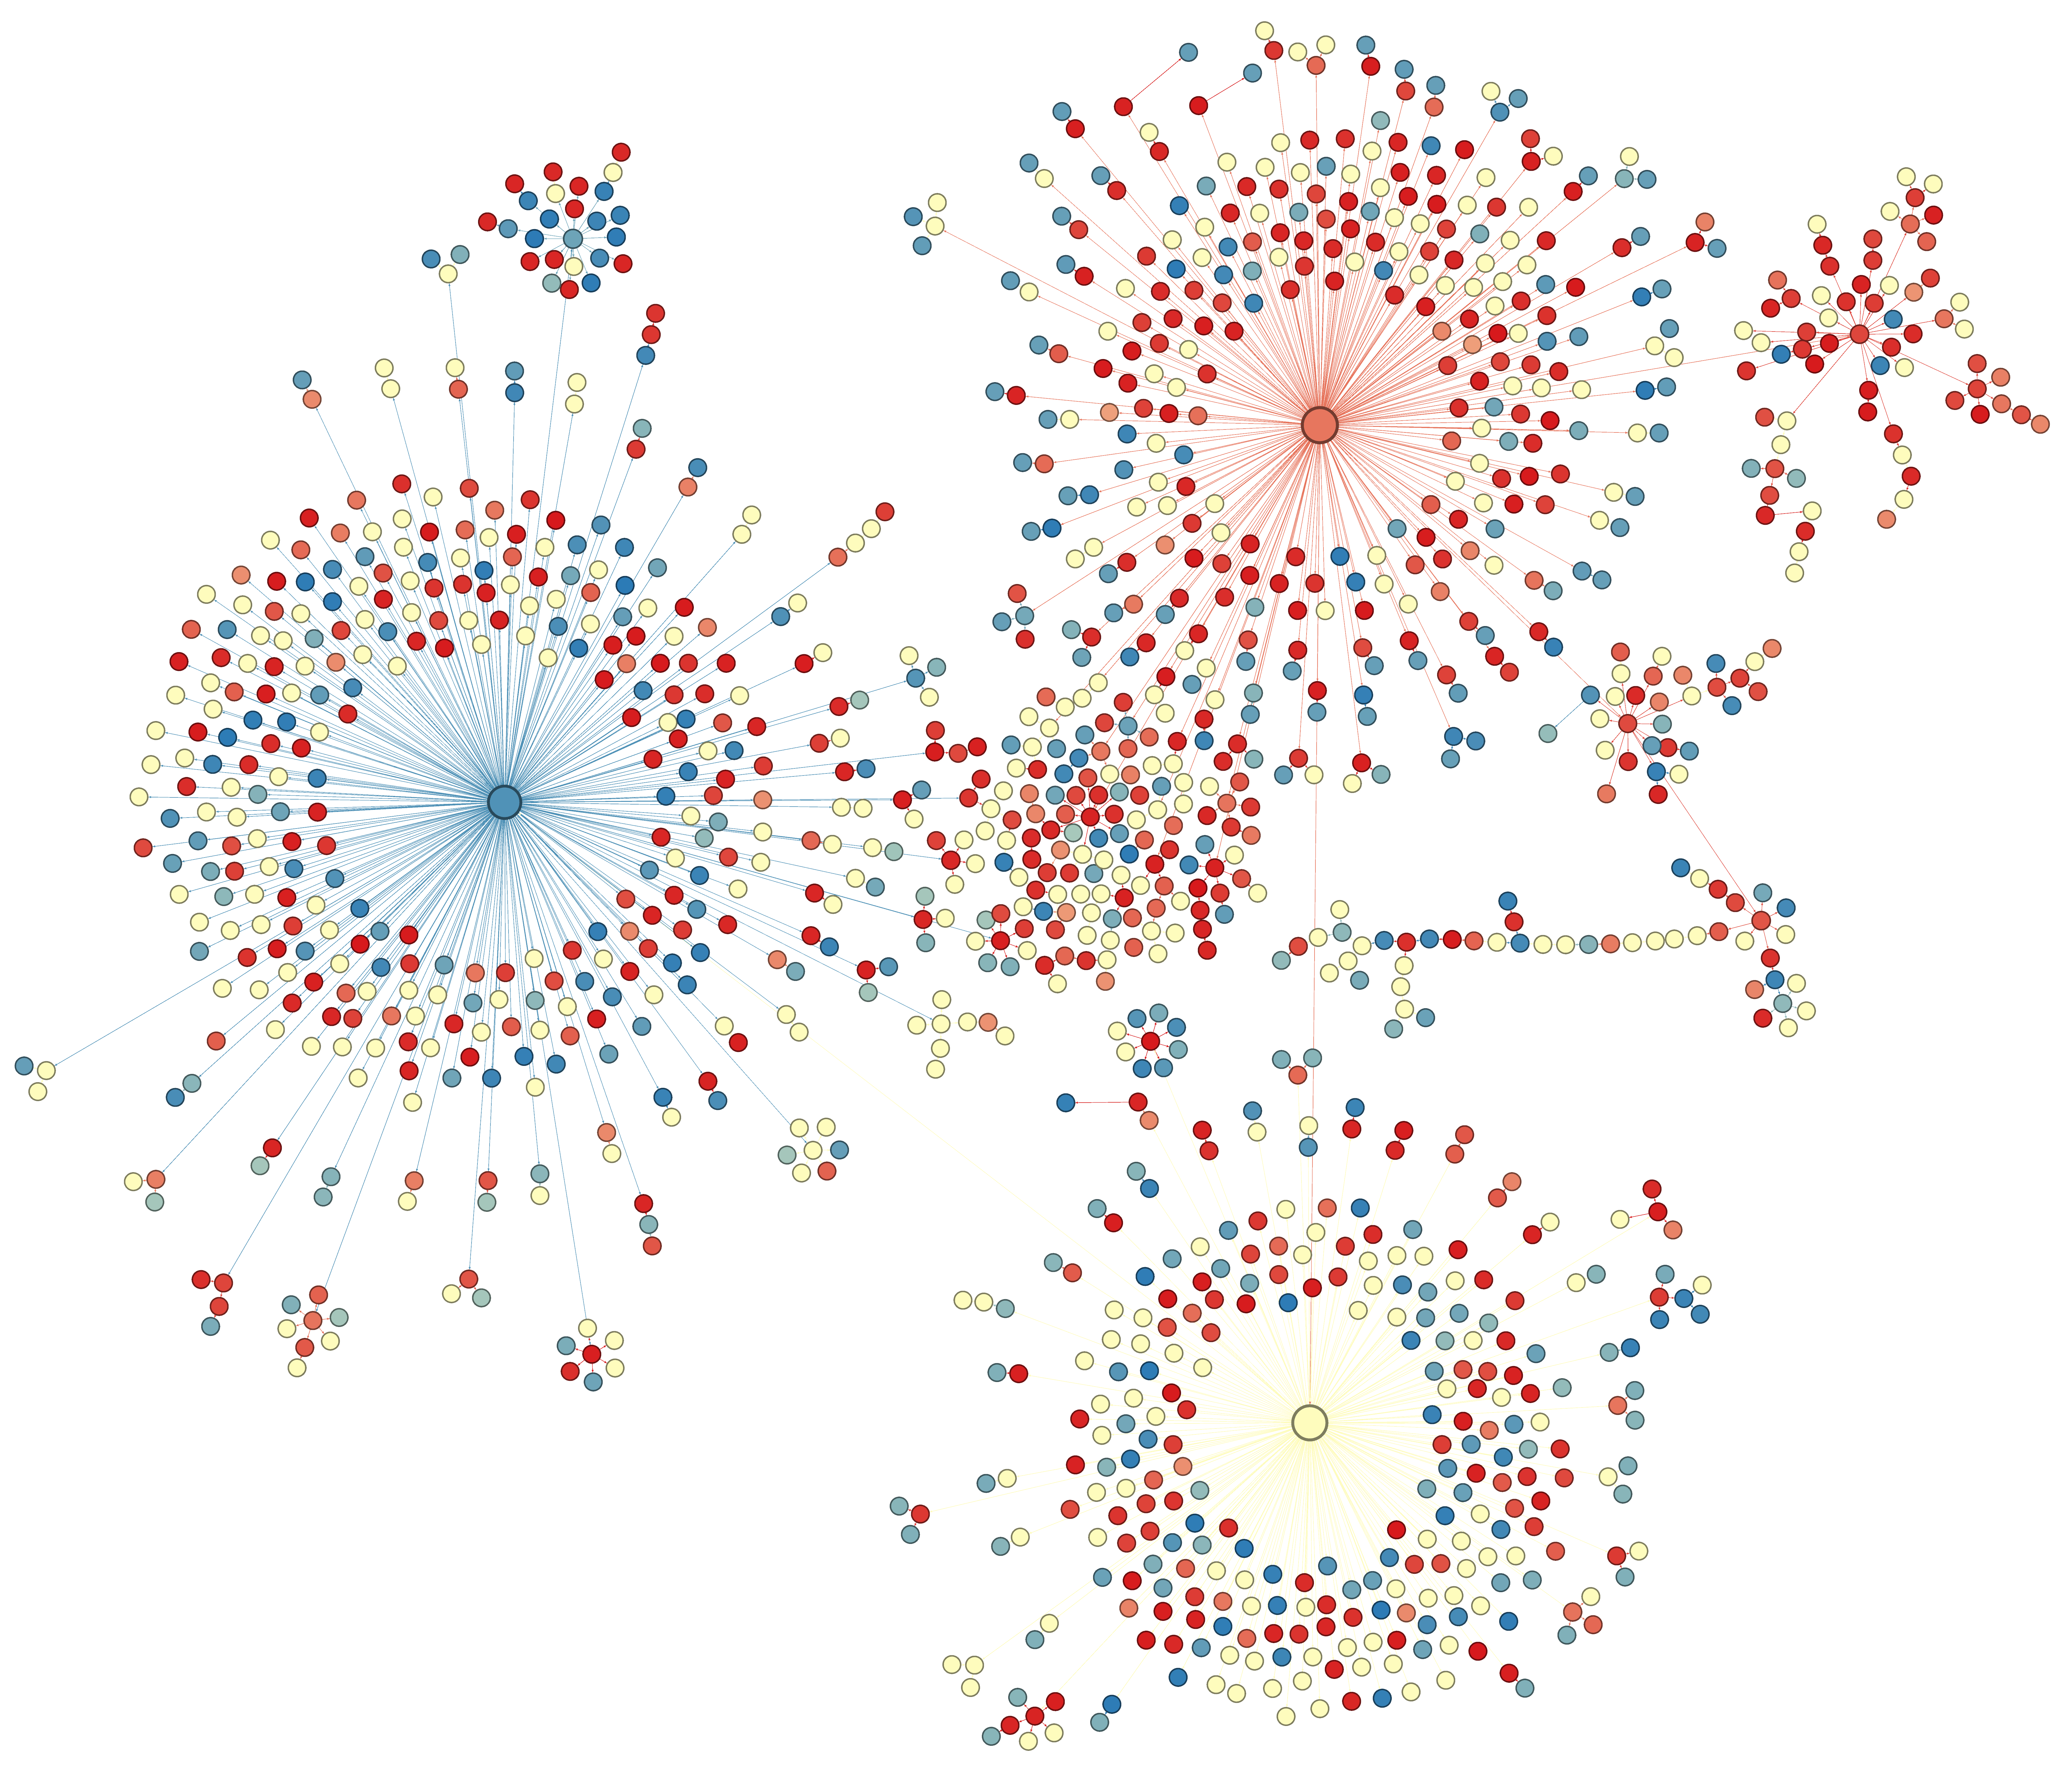
\includegraphics[width=\textwidth]{./figures/Results/graph/tweet-reply-weak-6.png}};

						\node[tweettext,callout relative pointer={(1.5em,-3.5em)},text width=8em] (n1text)
						at ($(maingraph.north west) + (5em, -6em)$)
						{As regulatory frameworks are developed and as the industry continues to evolve toward greater decentralization, the ecosystem will grow stronger.};

						\node[tweettext,callout relative pointer={(-3em,-4em)}] (n2text)
						at ($(maingraph.north east) + (-9em, -1em)$)
						{In the beginning, our hope was to be able to support FTX’s customers to provide liquidity, but the issues are beyond our control or ability to help.};

						\node[tweettext,callout relative pointer={(4em,0.5em)}] (n3text)
						at ($(maingraph.south west) + (9em, 4em)$)
						{Every time a major player in an industry fails, retail consumers will suffer. We have seen over the last several years that the crypto ecosystem is becoming more resilient and we believe in time that outliers that misuse user funds will be weeded out by the free market.};

						\node[rectangle,align=center,text width=0.8\textwidth] (description)
						at ($(maingraph.south)+(0,-0.7em)$)
						{\footnotesize
							\color{rpi_darkgray}
							\centering
							7\textsuperscript{th} largest weakly connected component in \textbf{relply} network.\\
							The three central tweets are from a single thread by Changpeng Zhao, former CEO of Binance.
						};

					\end{tikzpicture}
				\end{minipage}%
				\begin{minipage}[t]{.49\textwidth}%
					% \vspace{1em}

					\centering
					\begin{figure}
						\centering
						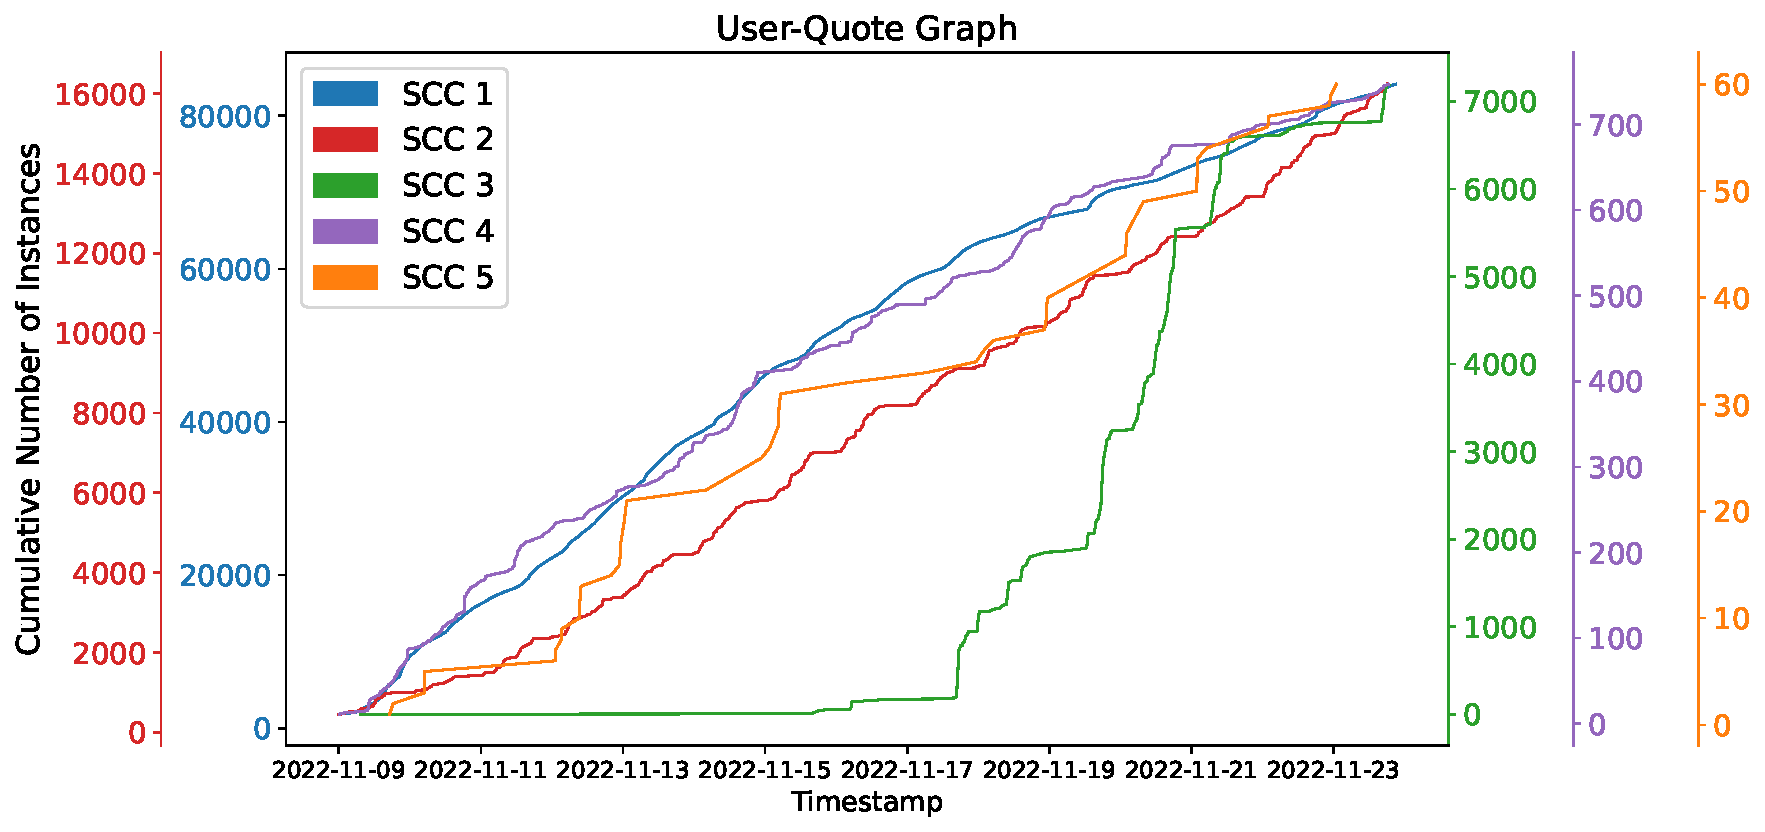
\includegraphics[width=.7\textwidth]{./figures/Results/graph/user_quote_scc_evolution.pdf}
					\end{figure}

					\begin{figure}
						\centering
						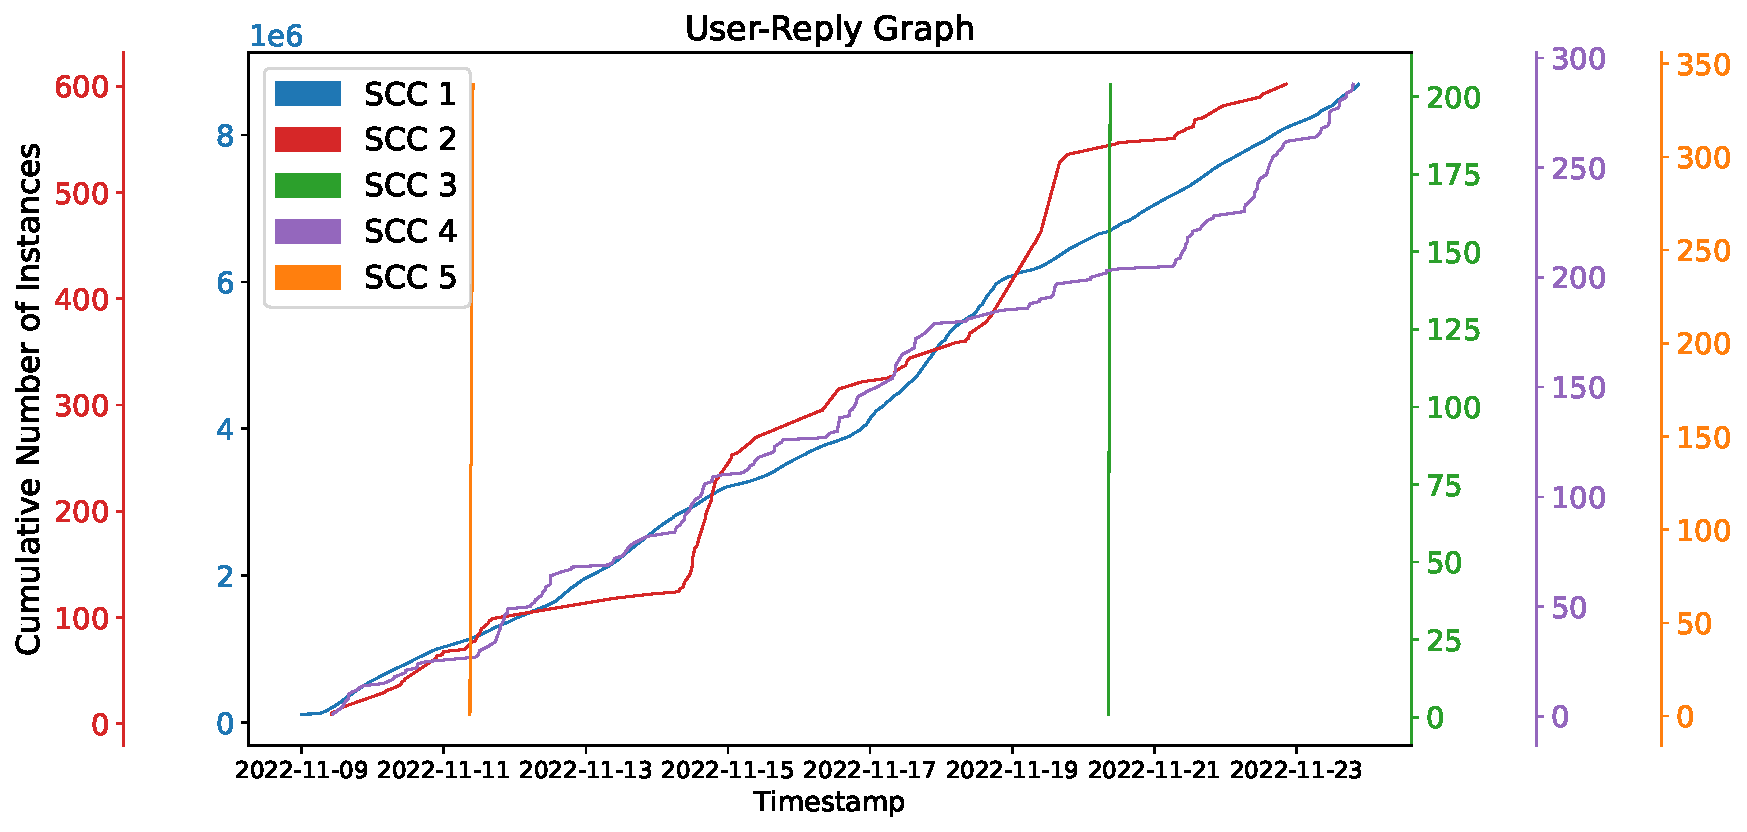
\includegraphics[width=.7\textwidth]{./figures/Results/graph/user_reply_scc_evolution.pdf}
					\end{figure}
					{\color{rpi_darkgray} \small Change in SCC component size for user networks.}

					{
					\begin{itemize}
						\item \textbf{Heavy influencer presence} (Professional Athletes, Tech Influencers, Meta-Commenters, etc.).
						\item \textbf{Obesrvable pattern} of bot-suspicious accounts.
						\item Identifiable network of \textbf{bot-suspicious accounts boosting} each other's presence.
						\item \textbf{Propgation} of negative/positive sentiment.
						\item Identification of potential \textbf{market manipulation attempts}.
					\end{itemize}
					}
				\end{minipage}%
			\end{block}
		\end{column}
		\begin{column}{0.01\paperwidth}\end{column}
	\end{columns}
\end{frame}
\end{document}
